\documentclass[runningheads]{llncs}
\usepackage[T1]{fontenc}
\usepackage{graphicx}
\usepackage{subfiles}
\usepackage[nolist]{acronym}
\usepackage[backend=biber,style=numeric,]{biblatex}
\usepackage[english=american]{csquotes}
\usepackage{hyperref}
\usepackage{color}
\usepackage{amssymb}
\usepackage[fleqn,tbtags]{mathtools}
\usepackage{minted}
\usepackage{amsmath}
\usepackage{nccmath}
\usepackage{caption}
\usepackage{algorithm}
\usepackage{algpseudocode}
\usepackage{subcaption}
\usepackage{xcolor} % to access the named colour LightGray
\definecolor{LightGray}{gray}{0.9}
\addbibresource{literatur.bib}
% alter autoref visualization
\def\sectionautorefname{Section}
% subfig setup
\usepackage[labelformat=simple]{subfig}
\renewcommand\thesubfigure{(\alph{subfigure})}
\renewcommand{\subfigureautorefname}{\figureautorefname}

\newcommand*\betreuerIES{Christian Gruhl }
\newcommand*\authorFF{W. Hilal \acfi{etal}}

\renewcommand*\contentsname{Inhaltsverzeichnis}
\renewcommand*\listfigurename{Abbildungsverzeichnis}
\renewcommand*\listtablename{Tabellenverzeichnis}
\newcommand\algorithmautorefname{Algorithm}

\algtext*{EndWhile}% Remove "end while" text
\algtext*{EndIf}% Remove "end if" text
\algtext*{EndFor}% Remove "end for" text

\begin{document}

\title{Identifying fiscal fraud with anomaly detection techniques}
\author{Klara M. Gutekunst}
\institute{University of Kassel, 34125 Kassel, Germany
\email{klara.gutekunst@student.uni-kassel.com}}

\maketitle
\begin{abstract}
This survey addresses the task of identifying fiscal fraud using anomaly detection techniques with regard to the problem governments' tax offices are facing in terms of tax evasion. As it is difficult to find profound studies of this specific problem, papers about a transferable problem are used to identify different approaches to face the original problem.
Multiple supervised methods to tackle credit card fraud are listed. 
The main focus of this survey is on unsupervised techniques. 
The four methods \acl{ARIMA}, \acl{IF}, \acl{AE}, and \acl{SOM} are described in more detail. 
This paper provides a discussion on how applicable each of these approaches is to the original problem, as well as a short outline of the approaches' shortcomings.

\keywords{unsupervised learning \and anomaly detection \and fiscal fraud \and fraud detection}
\end{abstract}
\section{Introduction}
Due to the fact, that a lot of monetary transactions happen via credit cards, the potential for fraudulent actions in this domain is increasing. 
Since these fraudulent actions result in great loss of money for credit card owners or companies, this topic has become a priority and many data scientists have started focussing their research on fiscal fraud detection.
While detection of fraudulent credit card actions may happen in real-time, fiscal fraud detection in tax offices is offline\footnote{According to \cite{gruhl2022}, an algorithm works in an offline fashion, if it requires access to the complete data set at once to perform a successful detection.}. Although tax evasion does not directly affect individuals, but the government, techniques of credit card fraud detection may be adapted to identify tax evasion. 
The goal of this survey is to outline four of the ways researchers have already found to identify financial fraud with unsupervised techniques.

The remainder of this article is structured as follows. 
First, the problem at hand is discussed in \autoref{sec:problem}. After that in \autoref{sec:state_of_art}, the existing techniques for a transferable anomaly detection problem are briefly listed. In \autoref{sec:main_part}, four unsupervised techniques are described in more detail. Afterwards, these techniques are compared in a discussion about their potential with regard to the problem at hand. Finally, there is a conclusion and outlook.

\section{Problem}
\label{sec:problem}
A government's tax office has various ways to detect fraudulent activities of companies that deliberately take actions to pay fewer taxes than they are supposed to pay. One way of detecting fraudulent activities is using the cash register data of companies to identify anomalies, which is currently performed by humans.
Data mining techniques can support this process.

The cash register of a business is supposed to log every transaction and thus, is a valuable resource for analysing the business' finances.
The data's structure depends on the cash register system. 
The documentation of an exemplary cash register's data structure is given in \cite{Vectron}. Every transaction is logged with attributes such as \texttt{date}, \texttt{time}, \texttt{clerk}, \texttt{identification}, and \texttt{item}. 
When exporting the data it is partitioned and stored in different files which are linked via keys.

Some systems have data subsets that are redundant, due to the fact that there are data files considered fiscally ir-/relevant. In this context, it is important to investigate both data subsets considered fiscally ir- and relevant, since it is possible that some anomalies are only evident in files consisting of non-aggregated entries, which may be considered fiscally irrelevant according to the documentation of the cash register system.

The structures of data sets from different cash register systems usually have some similarities, since there are standards for cash register data set by the \acfi{IFRS} according to \cite{ff_review_techniques}.
One similarity in any cash register data set is periodic behaviour, for instance in features such as \texttt{time of transaction}. A hypothesis regarding the data is that there are similarities between weekday data over months.

\section{State of the art}
\label{sec:state_of_art}
In this section, technical terms specific to the domain are defined and briefly discussed.
Moreover, the structure of feasible credit card data is outlined.
In the end, a brief overview of some of the financial fraud detection techniques is provided.

\subsubsection{Financial fraud:}
Financial fraud may be defined by \textquote[from \cite{ff_review_techniques}, based on \cite{acfe_ff}]{any intentional act to deprive another of property or money by guile, deception, or other unfair means}.
There are several different types of financial fraud, for instance, money laundering, credit card or insurance fraud as listed in \cite{ff_review_techniques}.
This survey's focus is on credit card fraud, since its detection techniques can be transferred to the problem presented in \autoref{sec:problem}.
According to \cite{ff_review_techniques} there are multiple types of credit card fraud including application fraud\footnote{identity fraud to issue new cards from credit companies} and behavioural fraud (unauthorised usage of credit cards by third parties, bankruptcy fraud\footnote{filing for personal bankruptcy instead of paying back the balance}).


\subsubsection{Anomalies:}
There is no general definition of an \textit{anomaly}. However, the authors of \cite{ff_review_techniques} use the definition of Hawkins, which identifies outliers or anomalies as observations which deviate so much from the other observations as to arouse suspicions that they were generated by a different mechanism. There are three different types of anomalies, which are examined in \cite{gruhl2022, ff_review_techniques}.

\textit{Point anomalies} are single instances of the data, which deviate from the rest of the data set. They can occur in any data set.

There are \textit{contextual} and \textit{behavioural} attributes. For instance, \texttt{time} in time-series data describes the context of that data and is therefore a \textit{contextual} attribute. Regarding this example from \cite{ff_review_techniques}, the attribute \texttt{temperature} is a non-contextual attribute and thus, is a \textit{behavioural} attribute.
\textit{Contextual anomalies} are individual instances which deviate in terms of the \textit{behavioural} attribute in a specific context. For instance, the temperature of a certain month is exorbitant greater than the ones documented in the respective months in other years. These anomalies can only occur if there are contextual attributes in the data.

Moreover, Gruhl discusses \textit{collective} anomalies or so-called \textit{novelties}, which are multiple data instances, whose occurrence as a group is anomalous with respect to the whole data set, in \cite{gruhl2022}. They can only occur if there is a relationship between the data instances.


\subsubsection{Challenges of Anomaly Detection:}
Anomaly detection is challenging due to a variety of reasons pointed out in \cite{gruhl2022, ff_review_techniques}.
Firstly, there are numerous types of normal behaviourism and therefore, it is difficult to consider all of them when classifying an individual instance. Respectively, anomalous individuals may differ greatly in their characteristics as they are irregular.
Moreover, the boundary between normal and anomalous individuals often lacks precision. 
It is difficult to determine, since the underlying model of normal data may change over time.
Another issue when dealing with anomaly detection tasks is the lack of labelled data for training as a consequence of the costly and time-consuming nature of this task.
Given that there is usually some degree of natural noise in the data, it is difficult to distinguish between noise and actual anomalies.
One also has to consider changing the data set's dimension. However, certain relations or anomalous behaviours may be evident in a certain dimension but become hidden after a dimension reduction.


\subsubsection{Data labels:}
The goal of anomaly detection is to assign a label to every instance of a data set indicating whether it is an anomaly or not.
In some cases, there are already labels present for a portion of the data set.
As stated in \cite{ff_review_techniques}, there are different types of anomaly detection techniques which either require labelled data (semi-/supervised) or not (unsupervised).


\subsubsection{Credit card data:}
Credit card data may be stored as a file containing $n$ features, such as \texttt{time}, \texttt{amount}, \texttt{id}, for $m$ transactions. 
Each transaction $t_i$ has a unique id $i$.
The data sets are highly imbalanced.
There is data available online, for instance on kaggle, however, due to confidentiality issues, the data from \cite{kaggle_ex} is not provided in its original form.
In this case, \acfi{PCA} transformation was used on all features except \texttt{time} and \texttt{amount}.
Originally, credit card data may contain non-numeric features.
Depending on the context, credit card data contains transactions of one or multiple individuals.
Hence, in some cases, the data is considered a time series.


\subsubsection{Models and techniques:}
Data preprocessing is important, since, for instance (supervised) machine learning techniques ignore minority classes in imbalanced data sets and thus, perform poorly on them.

According to \cite{ff_profiles}, cardholder profiles are created based on the cardholders' spending behaviours and patterns in order to detect credit card fraud. Abnormal transactions, such as drawing out unusually large amounts of money from inconvenient locations, may indicate fraudulent actions.

As stated in \cite{ff_review_techniques}, models used for identifying credit card fraud include \textit{\aclp{DT}} (\acs{DT})\acused{DT}, \acfi{SVM}, \acfi{LR} and \acfi{kNN}, which are outlined in \cite{sahin2010detecting}. It is also possible to combine those models in an ensemble along the lines of the \acfi{RF} algorithm.
Frequently used deep learning anomaly detection techniques and architectures are \acfi{NN}, \acfi{CNN}, \acfi{LSTM}, \textit{\aclp{AE}} (\acs{AE})\acused{AE} and \acfi{GAN}.
The models and techniques stated above are outlined in \cite{ff_review_techniques}.

The unsupervised financial fraud detection techniques \acfi{IF}, \acfi{AE}, \acfi{ARIMA}, \acfi{SOM}, which form the basis of this survey and are respectively described in \cite{liu2008isolation, cf_AE, fd_ARIMA, fd_SOM, credit_f_SOM}.

\section{Main part}
\label{sec:main_part}
Since it is most applicable to the problem presented in \autoref{sec:problem}, this section only focuses on unsupervised anomaly detection techniques.
The remainder of this paper concentrates on transferable problems, such as credit card fraud, because there are more scientific papers covering these problems.

\subsection{Isolation Forest}
The goal of this approach is to isolate anomalies from the normal data. The paper \cite{liu2008isolation} describes and evaluates this approach using multiple different data sets.
Based on the hypothesis that anomalies stand out with regard to the values of their attributes, they are identified by the small number of separations necessary to isolate them in the process of recurrent sub-sampling of the data set.

The concept of binary trees is essential for the technique \acfi{IF}.
Every node is either an external or internal node with no or respectively two children. 
Children of a node correspond to a partition of the parent node's data set.

A tree is constructed as follows:
\begin{enumerate}
    \item root of tree $\coloneqq$ data set $X$; $\psi \coloneqq$ sub-sampling size $\widehat{=}$ $|X|$
    \item A parent node $T$, has two children nodes $T_l, T_r$, a test attribute $q$ and a split value $p$
    \begin{enumerate}
        \item $q$ is randomly selected from existing attributes
        \item $p$ is randomly selected within minimum and maximum value of $q$
        \item $T_l \coloneqq \{x \mid x \in X \wedge x[q] < p\}$
        \item $T_r \coloneqq \{x \mid x \in X \wedge x[q] \ge p\}$
    \end{enumerate}
    \item Recursively divide $X$ into sub-samples $X_i$, until either
    \begin{enumerate}
        \item The tree reaches the height limit $l \coloneqq \lceil \log_2 \psi \rceil$
        \item $\vert X_i \vert = 1$
        \item All data in $X_i$ have the same values
    \end{enumerate}    
\end{enumerate}

According to \cite{gruhl2022, liu2008isolation} the characteristics of the constructed trees are:
\begin{enumerate}
    \item $n \coloneqq$ number of external nodes of an \acfi{iTree}
    \item $n-1$ internal nodes in an \ac{iTree}
    \item $h_i(x) \coloneqq $ number of edges from root node to external node $x$ $\widehat{=}$ Path length in \ac{iTree} $i$
    \item $t \coloneqq$ total number of \acp{iTree}
    \item $\bar {h(x)} \coloneqq \frac{1}{t}\sum_{i=1}^{t}h_i(x)$ $\widehat{=}$ average path length of $x$ 
    \item $c(\psi) \coloneqq $ average path length of a binary tree for a given sample set of $\psi$ observations
    \item $s(x, \psi) \coloneqq 2^{-\frac{\bar {h(x)}}{c(\psi)}}$ $\widehat{=}$ anomaly score 
    \begin{enumerate}
        \item $\bar {h(x)} \to c(\psi) \Rightarrow s \to 0.5$
        \item $\bar {h(x)} \to 0 \Rightarrow s(x, \psi) \to 1$ $\widehat{=}$ $x$ is an anomaly
        \item $\bar {h(x)} \to n-1 \Rightarrow s(x, \psi) \to 0$ $\widehat{=}$ $x$ is a normal instance
    \end{enumerate}
\end{enumerate}
%
\begin{figure}
    \begin{subfigure}[t]{0.23\textwidth}
        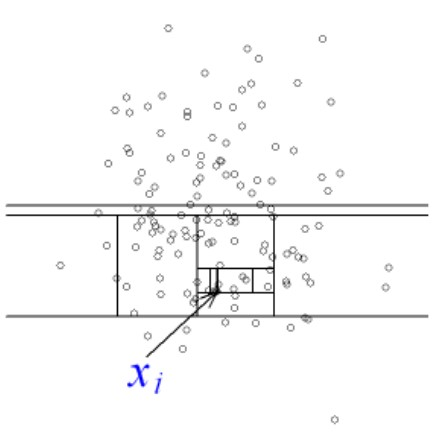
\includegraphics[width=1\textwidth]{images/IF_isolate_normal_inst.jpg}
        \caption{Normal instance}   
        \label{fig:IF_isolate_normal_inst}
    \end{subfigure}
    \begin{subfigure}[t]{0.23\textwidth}
        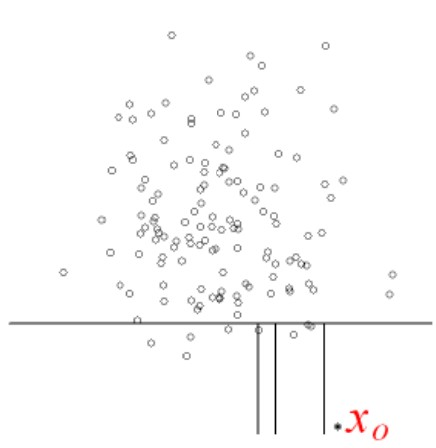
\includegraphics[width=1\textwidth]{images/IF_isolate_abnormal_inst.jpg}
        \caption{Anomaly $x_0$}
        \label{fig:IF_isolate_abnormal_inst}
    \end{subfigure}
    \begin{subfigure}[t]{0.23\textwidth}
        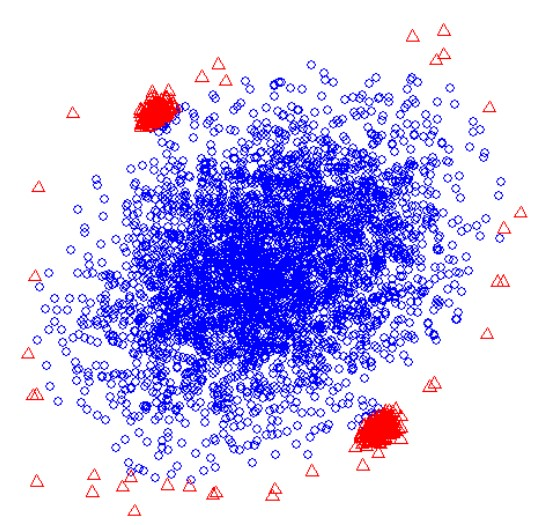
\includegraphics[width=1\textwidth]{images/IF_original_sample.jpg}
        \caption{Original data}   
        \label{fig:IF_original_sample}
    \end{subfigure}
    \begin{subfigure}[t]{0.23\textwidth}
        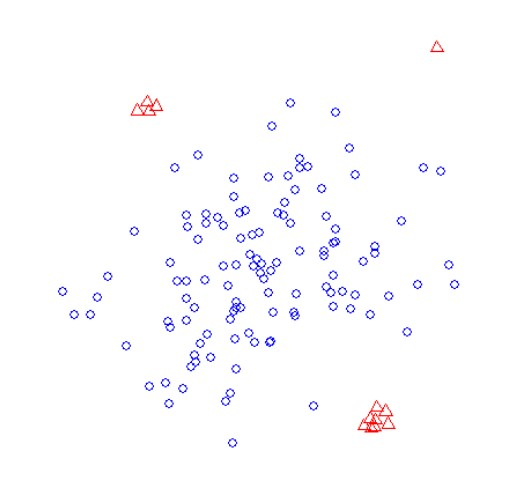
\includegraphics[width=1\textwidth]{images/IF_subsample.jpg}
        \caption{Sub-sample}
        \label{fig:IF_subsample}
    \end{subfigure}
    \caption{Visualisation of instance isolation and sub-sampling from \cite{liu2008isolation}. 
    The normal instance $x_i$ in \autoref{fig:IF_isolate_normal_inst} requires more partitions (visualised by horizontal and vertical lines) to be isolated than the anomaly $x_0$ in \autoref{fig:IF_isolate_abnormal_inst}, due to $x_0$'s solitary position.
    In \autoref{fig:IF_original_sample} for the original data and \autoref{fig:IF_subsample} for a sub-sample of the original data, blue circles denote normal instances, whereas red triangles denote anomalies. Anomalies are isolated quicker in less dense data sets such as \autoref{fig:IF_subsample}.}
\end{figure}
%
The approach is based on the hypothesis, that anomalies are less frequent (a minority in the data set) and have attribute values that extremely deviate from those of normal instances. 
Based on this hypothesis, the authors of \cite{liu2008isolation} conclude, that anomalies, as depicted in \autoref{fig:IF_isolate_abnormal_inst}, require fewer partitions to be isolated than normal instances of a data set, which is visualised in \autoref{fig:IF_isolate_normal_inst}. 
The number of partitions required to isolate a data point is equal to path length $h_i(x)$ in an \ac{iTree} $i$. 
Hence, an average path length of $\bar {h(x)} \to 0$ suggests that the grand majority of the \acp{iTree} has short paths from the root to the instance $x$ and thus, consider $x$ an anomaly.

Anomalies are identified as nodes having shorter path lengths, which means they are isolated earlier than normal instances. 
Hence, the process of dividing the data set into sub-samples can be terminated at the tree height limit $l$, since the anomalies should be isolated by then. 
However, not all normal instances are isolated at this point and thus, a partial model is created.
If a data point $x$ belongs to the part of the tree, which was not built, because for instance, the tree height limit $l$ has been reached and thus, expansion was terminated, an adjustment account $c(\text{size of unbuilt subtree})$ is added when calculating its path length.

Since \acp{iTree} work well if the sampling size is kept small, sub-sampling is conducted. Comparing \autoref{fig:IF_original_sample} and \autoref{fig:IF_subsample}, it becomes clear that fewer data points are favourable to the isolation technique since they are less dense and thus, anomalies are more likely to be isolated early.

According to \cite{liu2008isolation}, swamping refers to wrongly identifying normal instances as anomalies. Masking is the existence of too many anomalies concealing their own presence. Both problems arise from too much data. \acp{iTree} build a partial model by sub-sampling and thus, control the data size and specify on a sub-sample of anomalies or respectively a lack of them. 

Anomaly detection using \acp{IF} is a two-stage process. 
As stated in \cite{gruhl2022, liu2008isolation}, first, in the training stage, sub-samples of size $\psi$ from the training set are used to build \acp{iTree}. 
Then, in the evaluation stage, test instances are passed through the \acp{iTree} to obtain anomaly scores based on their path length. 
The highest $m$ anomaly scores correspond to the $m$ anomalies identified by the \ac{IF}. 

The input parameter $\psi$ controls the input data size in the training stage whereas the number of trees $t$ controls the ensemble size. 
Empirical studies from \cite{liu2008isolation} suggest that $\psi = 2^8 = 256$ and $t = 100$ are optimal to perform anomaly detection across a wide range of data.
Owing to the fact that there are multiple \acp{iTree} it is called a forest. 
Obviously, multiple \acp{iTree} have different sets of partitions, due to the fact that they are randomly generated.
\subsection{Autoencoder}

The idea of the approach is to use a low-dimensional version of the data to identify anomalies either using a trained model or the reconstructing error when reconstructing the encoded data.
The approach from \cite{cf_AE} consists of two stages. 
Firstly, the dimension of the high-dimension credit card data is reduced using an undercomplete \acfi{AE}, which is a feed-forward neural network depicted in \autoref{fig:AE_Aufbau} that learns efficient (non-correlated) encodings for the input data. It is called undercomplete because the dimension of its hidden layer, or so-called latent space, is smaller than the dimension of the input layer. Feed-forward means that after training the information moves in only one direction (forward) and thus, no loops or cycles exist. However, while training, the network employs backpropagation\footnote{updating weights and biases of the neurons based on forward propagation error} to update the parameters.
%
\begin{figure}[http]
    \begin{center}
      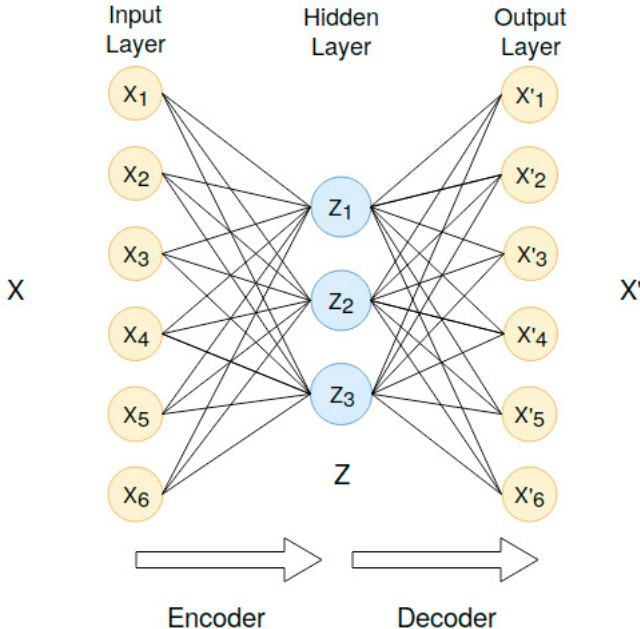
\includegraphics[scale=0.3]{images/AE_Aufbau.jpg}
      \caption{Structure of \ac{AE} from \cite{cf_AE}}
      \label{fig:AE_Aufbau}
    \end{center}
\end{figure}

The goal of an \ac{AE} is to approximate the identity function $f_\theta(X) = X$ (trivial solution eliminated) for input $X$ and function parameters to be learned $\theta$.
The input and output layer have the same dimension since the encoded data is reconstructed in the output layer. 

The mathematical background of the encoder is given in \eqref{eq:encoder}. The dimension reduction is computed using weight $W_\theta$, bias $B_\theta$ of the encoder layer, and the (non-)linear encoder activation function $f_E(.)$. Owing to the usage of a non-linear activation function, the neural network is capable of more than linear regression.
%
\begin{ceqn}
    \begin{equation}
    \label{eq:encoder}
        Z = f_E(W_\theta X + B_\theta)
    \end{equation}
\end{ceqn}
%
The decomposition of the reduced dimensionality data to the output $X'$ is calculated analogously to \eqref{eq:encoder}. \eqref{eq:decoder} is used for the decoder.
%
\begin{ceqn}
    \begin{equation}
    \label{eq:decoder}
        X' = f_D(W_\theta Z + B_\theta)
    \end{equation}
\end{ceqn}
%
The Euclidean distance from \eqref{eq:recon_err} between the input $X$ and the output $X'$, which is reconstructed from $Z$, is considered the reconstruction error. According to \cite{AE_RF}, error backpropagation and gradient descent\footnote{iterative algorithm to find the function’s coefficients that minimise the corresponding cost function using derivatives and the learning rate} are employed to train the \ac{AE} with the goal of minimising the reconstruction error. The reconstruction error can be used to identify anomalies: If the reconstruction error is greater than a certain threshold\footnote{e.g. iterative computation of the threshold value analogously to \autoref{alg:AE_PRF}}, $X$ is considered an anomaly based on the hypothesis that the \ac{AE} has approximated the identity function for normal instances.
%
\begin{ceqn}
    \begin{equation}
    \label{eq:recon_err}
       \triangle (X, X') = \parallel X - X' \parallel_2
    \end{equation}
\end{ceqn}
%
To avoid overfitting, a regulariser tuning the objective function of the learning algorithm may be added.

The approach from \cite{cf_AE} first uses the encoder, which transforms $X$ to $Z$. Since the authors assume that $X$ can be reconstructed using $Z$, it is a valid representation of the input transaction.
Then, a classifier is trained on $Z$. In \cite{cf_AE} labelled transactions of a training set are used to train a \acfi{MLP}, \acfi{kNN}, \acfi{LR}, but generally, every model can be used to identify anomalies. 
%
\begin{algorithm}
\caption{\acfi{AE-PRF}}\label{alg:AE_PRF}
 \hspace*{\algorithmicindent} \textbf{Input:} training data $D_{train}$,  validation data $D_{val}$, test data $D_{test}$, metric $M$ \\
 \hspace*{\algorithmicindent} \textbf{Output:} classification of each instance (0 if normal, 1 else)

\begin{algorithmic}[1]
\State Train the \ac{AE} model $\ac{AE}_T$ with $D_{train}$
\Comment{pseudocode based on \cite{AE_RF}}
\State $T \gets \ac{AE}_T(D_{train})$
\Comment{$T$ set of training data after dimension reduction}
\State Train the \ac{RF} model $\ac{RF}_T$ with $T$
\State $V \gets \ac{AE}_T(D_{val})$
\Comment{$V$ set of validation data after dimension reduction}
\For{$\theta \gets 0$ \texttt{to} $1$ \texttt{step} $0.01$}
\Comment{iterative testing of possible threshold values $\theta$}
    \For{$v \in V$}
        \State $p \gets \ac{RF}_T(v)$
        \Comment{probability $p$ of fraud classification}
        \If{$p > \theta$} 
            \State \texttt{result}$[\theta][v] \gets 1$
        \Else
            \State \texttt{result}$[\theta][v] \gets 0$
        \EndIf 
    \EndFor
\EndFor

\State Find best $\theta*$ by comparing all \textit{result} values in terms of metric $M$
\State $C \gets \ac{AE}_T(D_{test})$
\Comment{$C$ set of test data after dimension reduction}

 \For{$c \in C$}
        \State $q \gets \ac{RF}_T(c)$
        \If{$p > \theta*$} 
            \State \texttt{output}$[c] \gets 1$
        \Else
            \State \texttt{output}$[c] \gets 0$
        \EndIf 
    \EndFor

\State \textbf{return} \textit{output}
\end{algorithmic}
\end{algorithm}
%

\cite{AE_RF} proposes an \acfi{AE-PRF}, which is the combination of an \ac{AE} to extract transaction data features and a \ac{RF} with probabilistic classification to assign either the label fraudulent or normal to credit card transactions.
The approach \ac{AE-PRF} is illustrated in pseudocode in \autoref{alg:AE_PRF}.
The \ac{RF} in the paper is an ensemble learning model consisting of \acp{DT} and employs bagging\footnote{independently training multiple individual \acp{DT} based on random subsets of data and attributes}. In this case the \acp{DT}' internal nodes split the data set on the optimal (i.e. largest information gain) value of the corresponding split attribute. 
The splitting terminates if either all data of a node have the same value, the number of instances at a node reaches a predefined minimum limitation or the depth of the node reaches a predefined maximum limitation.
An instance is then passed through the tree and classified by an individual tree based on the label of its corresponding leaf. The final \ac{RF} classification of that instance is the result of a majority voting or averaging of the individual \acp{DT}, which have been constructed prior by using bagging.
The probabilistic classification requires an additional parameter threshold $\theta \in  [0,1]$. The \ac{RF} model classifies an instance as fraudulent with probability $p$ and respective as normal with probability $1 - p$. 
The final \ac{AE-PRF} classification of that instance is fraudulent if $p > \theta$ is true and normal otherwise.
The optimal threshold $\theta*$ can be determined by iterative testing of the classification performance in terms of a specific metric $M$ on different values for $\theta$.

\subsection{Autoregressive integrated moving average}

Based on the hypothesis that the \texttt{daily count of transactions} for a given customer for a certain point in time is correlated to some lagged values before that point in time, a model is trained using lagged values. Instances that deviate greatly from the predicted value of the trained model are considered fraudulent.
The approach \acfi{ARIMA} proposed in \cite{fd_ARIMA} is the combination of an \acfi{AR} model and a \acfi{MA} model. It frames the problem of credit card fraud detection as an anomaly detection task in time series, where the variable presented as the time series is the \texttt{daily count of transactions} for a given customer.

An \ac{AR} model assumes the value $X_t$ for time unit $t$ is based on the correlated lagged (i.e. previous) observations $X_{t-i}, 0 < i \le p$, a constant $c$ and an error term $\omega_t \sim  N(0, \sigma^2)$ as stated in \eqref{eq:AR}.
%
\begin{ceqn}
    \begin{equation}
    \label{eq:AR}
        X_t = c + \sum_{i=1}^p \phi_i X_{t-i} + \omega_t
    \end{equation}
\end{ceqn}
%
The coefficients $\phi = (\phi_1, ..., \phi_p)$ are estimated using the maximum likelihood estimation process.
The number of lagged observations $X_{t-i}$ to consider (i.e. the ones statistically relevant) is indicated by $p \in \mathbb{N}$, which is calculated using \acfi{PACF}.
%
\begin{ceqn}
    \begin{equation}
    \label{eq:pearson_corr}
        C(X,Y)=\sum_{i}^{}\frac{(X_i-\mu_X)(Y_i-\mu_Y)}{\sigma_X \sigma_Y}
    \end{equation}
\end{ceqn}
%
\ac{PACF} is graphically visualised in \autoref{fig:PACF_AR} by plotting the autocorrelation (Pearson correlation of $X_t$ with lagged observation of $X$ calculated in \autoref{eq:pearson_corr} from \cite{p_acf}) value on the y-axis and the lags ($t - i, 0 \le i$) on the x-axis. A data point displayed is the direct correlation of $X_t$ and $X_ {t-i}$ not taking into account the lagged observations $X_ {t-j}, 0 < j < i$: $C(X_{n+k},X_n|X_{n+k-1}, ..., X_{n+1})$.
The correlation values of lagged observations outside a certain threshold (illustrated by the blue confidence intervals) are considered statistically relevant.
%
\begin{figure}
    \begin{subfigure}[t]{0.5\textwidth}
        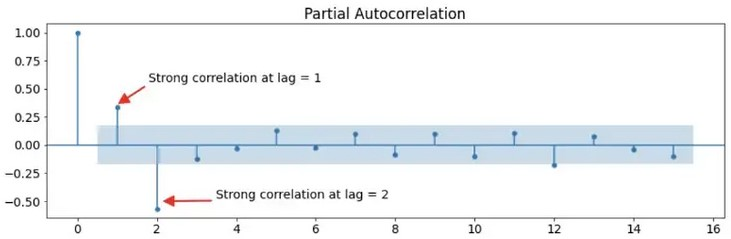
\includegraphics[width=1\textwidth]{images/PACF_AR(2).jpg}
        \subcaption{\ac{PACF} of \ac{AR}$(2)$}   
        \label{fig:PACF_AR}
    \end{subfigure}
    \begin{subfigure}[t]{0.5\textwidth}
        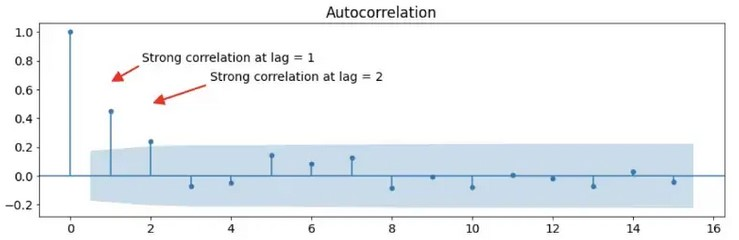
\includegraphics[width=1\textwidth]{images/ACF_MA(2).jpg}
        \subcaption{\acs{ACF} of \ac{MA}$(2)$}
        \label{fig:ACF_AR}
    \end{subfigure}
    \caption{Plots of two time series from \cite{P_ACF}. Values outside of the blue confidence interval are considered non-zero and thus, statistically relevant. \autoref{fig:PACF_AR}, \autoref{fig:ACF_AR} indicate respectively $p=2$, $q=2$.}
\end{figure}

A \ac{MA} model assumes the value $X_t$ for time unit $t$ is based on the correlated lagged (previous) errors $\omega_{t-j}, 0 < j \le q$, the mean of the series $\mu$ and an error term $\omega_t \sim  N(0, \sigma^2)$ as stated in \eqref{eq:MA}.
%
\begin{ceqn}
    \begin{equation}
    \label{eq:MA}
        X_t = \mu + \sum_{j=1}^q \theta_j \omega_{t-j} + \omega_t
    \end{equation}
\end{ceqn}
%
The calculation of the coefficients $\theta = (\theta_1, ..., \theta_q)$ is analogue to \ac{AR}.
This model assumes that the observations are located around the mean $\mu$, hence that the time series is stationary ($\mu, \sigma$ constant over time).
Thus, \eqref{eq:MA} without $\omega_t$ predicts $X_t$ based on the mean of the series and taking certain lagged errors $\omega_{t-j}$ into account. 
The error $\omega_t$ is added to calculate the real observation.
The number of statistically relevant lagged errors $\omega_{t-j}$ is indicated by $q$, which is calculated using an \acfi{ACF}.
\ac{ACF} is graphically visualised in \autoref{fig:ACF_AR} by plotting the autocorrelation value on the y-axis and the lags ($t - i, 0 \le i$) on the x-axis. It is important to note that a data point displayed is the indirect and direct correlation of $X_t$ and $X_ {t-i}$ calculated using \autoref{eq:pearson_corr}. Lagged observations considered statistically relevant are identified as stated above.
%
\begin{ceqn}
    \begin{equation}
    \label{eq:ARMA}
        X_t = c + \omega_t + \sum_{i=1}^p \phi_i X_{t-i} + \sum_{j=1}^q \theta_j \omega_{t-j} 
    \end{equation}
\end{ceqn}
%
The \acfi{ARMA} model in \eqref{eq:ARMA} is a combination of the \ac{AR} \eqref{eq:AR} and the \ac{MA} \eqref{eq:MA} models. The components are computed as stated above. However, the assumption of the \ac{MA} model, a time series is stationary, is not always true. Therefore, an \ac{ARIMA}($p, d, q$) model is constructed using the \ac{ARMA} model and the possibility of applying differencing of degree $d$ to data points to make them stationary (if necessary).

The Box-Jenkins method is used to tune the \ac{ARIMA} model. 
Firstly, the \acfi{ADF} test verifies if the time series is stationary.
The \ac{ADF} test rejects either hypothesis $H_0: \phi_i = 1 \Rightarrow \text{not stationary}$ or $H_1: \phi_i < 1 \Rightarrow \text{stationary}$.
Secondly, $p, q$ are configured as stated above.
Then, the training phase estimates coefficients $\phi, \theta$ as stated above.

\begin{figure}[http]
    \begin{center}
      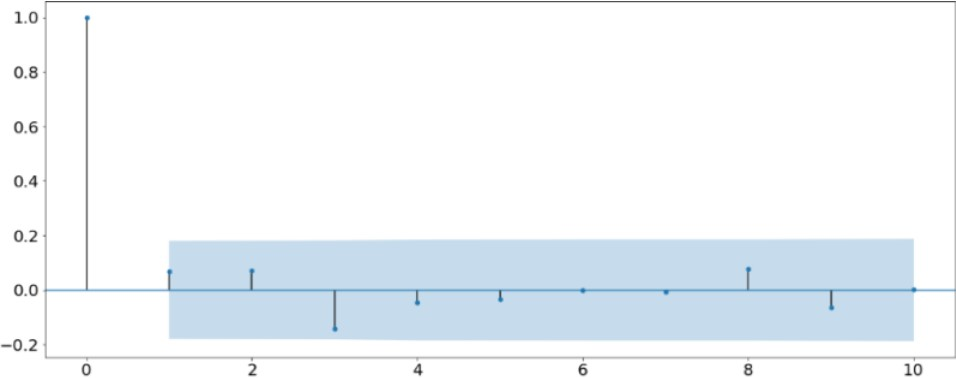
\includegraphics[scale=0.25]{images/ARIMA_correlogram_white_noise.jpg}
      \caption{Correlogram of residuals from \cite{fd_ARIMA}. A correlogram is the visualisation of the correlation of $X_t$ with lagged observations of $X$. Since none of the lagged residuals is considered statistically relevant, the model selected is optimal.}
      \label{fig:ARIMA_corr}
    \end{center}
\end{figure}

Lastly, the model is evaluated. For an ideal model, the error is normally distributed with mean $\mu$ of 0, constant variance $\sigma$ and the residuals are stationary (no temporal structure) as illustrated in \autoref{fig:ARIMA_corr}.

In order to detect fraudulent credit card transactions, the time series is split into a training (preferably only containing legitimate transactions) and testing set. 
The \ac{ARIMA} model is trained applying the Box-Jenkins method to the training set.
%
\begin{ceqn}
    \begin{equation}
    \label{eq:z-score}
        z = \frac{x-\mu}{\sigma}
    \end{equation}
\end{ceqn}
%
The fraudulent transactions of the testing set are identified by comparing the Z-score from \eqref{eq:z-score}, $x$ being the difference between predicted and actual \texttt{daily count of transactions}, $\mu, \sigma$ being the mean and variance based on the errors in predictions of the training set, with a certain threshold. A Z-score higher than the threshold corresponds to a fraudulent day.

\subsection{Self-organising map}
The goal of this approach is to identify fraudulent user accounts (i.e. bank accounts of individuals) using projection onto a two-dimensional feature space and a dissimilarity value.

The approach proposed in \cite{fd_SOM} is \acfi{SOM} as an example of artificial neural network architecture.
It has a feed-forward topology and unsupervised self-organising training algorithm discussed in \cite{credit_f_SOM}.

A record is a single transaction, which can be visualised as a vector (cf. single row in \eqref{eq:user_acc_matrix}). An entry of \eqref{eq:user_acc_matrix} corresponds to the value of the feature.
A user account is a set of records from one specific user. 
It is represented by the data matrix from \eqref{eq:user_acc_matrix}. 
$m$ is the number of features of a record and $n$ is the number of records, with $n \gg m$. 
Hence, $f_{i,j}$ is the $i$th value of the $j$th feature.
%
\begin{ceqn}
    \begin{equation}
    \label{eq:user_acc_matrix}
        \begin{pmatrix}
            f_{1,1} & ... & f_{1,m}\\
            ... & ... & ... \\
            f_{n,1} & ... & f_{n,m}
        \end{pmatrix}
    \end{equation}
\end{ceqn}
%
Unlike other financial fraud detection techniques, this approach uses data visualisation to identify fraudulent user accounts rather than individual transactions within a user account.

Since \acp{SOM} use vectors as input data, the matrices corresponding to a user account have to be transformed. This transformation or so-called projection of all features onto the \ac{SOM} is a dimension reduction $p$, where every original (high-dimensional) feature $f_j$ (with all inner-dimension entries $f_{i,j}, i \in [1, n]$, $n$ is number of records) is projected on a (2-dimensional) $\tilde f_j$ \eqref{eq:feature_projection}.
%
\begin{ceqn}
    \begin{equation}
    \label{eq:feature_projection}
        p: \mathbb{R}^n \to \mathbb{R}^2, f_j \mapsto \tilde f_j
    \end{equation}
\end{ceqn}

\begin{figure}
    \begin{subfigure}[t]{0.5\textwidth}
        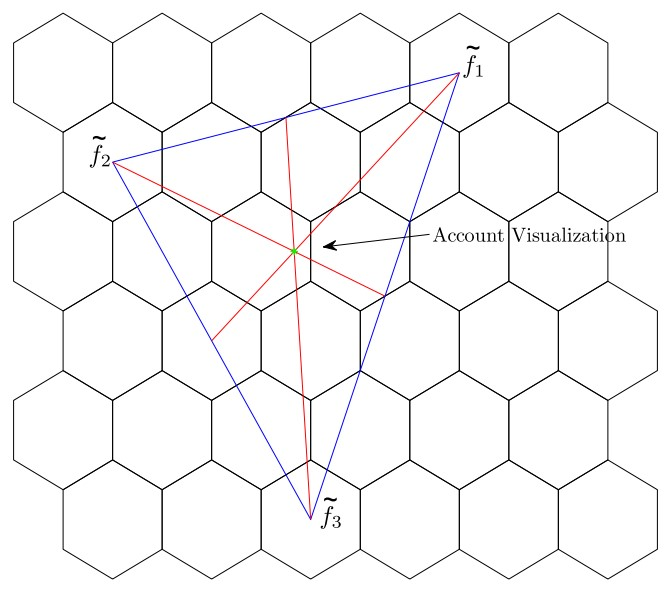
\includegraphics[width=1\textwidth]{images/SOM_user_acc_visualisation.jpg}
        \subcaption{User account representation}   
        \label{fig:SOM_user_acc_visualisation}
    \end{subfigure}
    \begin{subfigure}[t]{0.5\textwidth}
        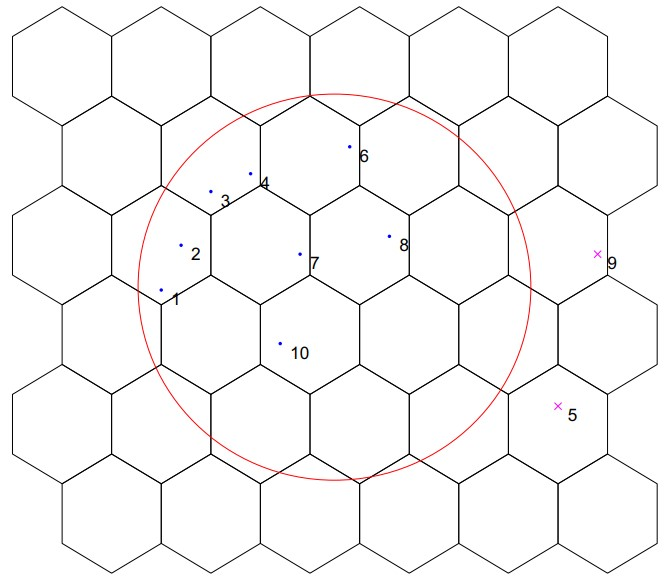
\includegraphics[width=1\textwidth]{images/SOM_threshold_bin_classification.jpg}
        \subcaption{Threshold-classification of instances}
        \label{fig:SOM_threshold_bin_classification}
    \end{subfigure}
    \caption{\ac{SOM} visualisation from \cite{fd_SOM}}
\end{figure}

The $i$th user account is represented by the centroid $c_i$ on the \ac{SOM} grid, which is calculated in \eqref{eq:acc_representation} and visualised in \autoref{fig:SOM_user_acc_visualisation}.
There can be accounts that do not correspond to a particular neuron (i.e. hexagon) in a \ac{SOM} grid. 
It is also possible that multiple similar accounts share a neuron.
%
\begin{ceqn}
    \begin{equation}
    \label{eq:acc_representation}
        c_i = \frac{1}{m}\sum^{m}_{j=1} \tilde f_{i,j}
    \end{equation}
\end{ceqn}
%
According to \cite{fd_SOM}, the reduction of the inner-dimensionality of features from \eqref{eq:feature_projection} does not reduce the amount of information, since the majority of records of a fraudulent user account are fraudulent themselves.

Each entry of the U-matrix of a \ac{SOM} corresponds to a neuron in the \ac{SOM} grid. Its value is the average dissimilarity between the neuron and its neighbours.
Hence, a so-called ridge (sequence of high values) in the U-matrix represents a borderline separating the data clusters in the corresponding \ac{SOM} grid.
\autoref{fig:U_Matrix} is a visualisation of an U-matrix. The colour of a hexagon corresponds to the value of the neuron in the U-matrix (cf. legend on the right side). 
Red coloured hexagons correspond to the highest values of average dissimilarity of neurons in the U-matrix. Hence, the group of red hexagons is a ridge. 
Although the closest user accounts below the ridge are considered non-fraudulent, the user accounts with more distance to the ridge (and below it) are marked as fraudulent. 
Thus, the ridge in fact separates the two clusters.

\begin{figure}[http]
    \begin{center}
      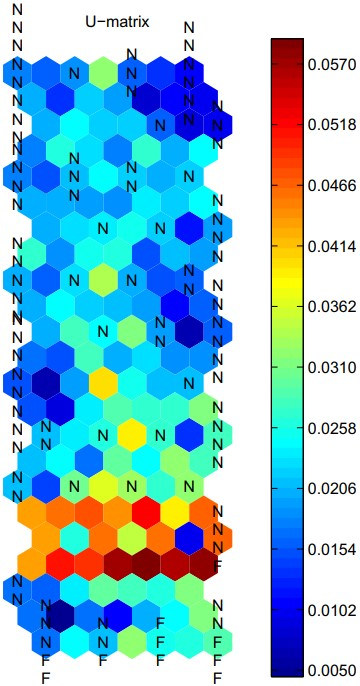
\includegraphics[scale=0.3]{images/SOM_U_Matrix_vis.jpg}
      \caption{Visualisation of U-matrix from \cite{fd_SOM}. The letter \textit{N} marks non-fraudulent user accounts, whereas \textit{F} marks fraudulent user accounts. The coloured hexagons correspond to the values of the average dissimilarity of neurons and their neighbours in the U-matrix.}
      \label{fig:U_Matrix}
    \end{center}
\end{figure}

As stated in \cite{fd_SOM}, the classification of (non-)fraudulent instances is performed by a threshold-type binary classification technique. 
Visually, the threshold of the circle illustrated in \autoref{fig:SOM_threshold_bin_classification} with centre $c$, which is the centroid of the entire \ac{SOM} grid and radius $\tau$, which is calculated in \eqref{eq:radius_threshold}.
$v_{max}$ is the \ac{SOM} neuron corresponding to the maximal value in the U-matrix of the \ac{SOM} and $d(.,.)$ is a chosen dissimilarity measure.
All points outside the circle are considered fraudulent user accounts and respectively all points within the threshold are considered normal user accounts.
%
\begin{ceqn}
    \begin{equation}
    \label{eq:radius_threshold}
        \tau = d(c, v_{max})
    \end{equation}
\end{ceqn}
%
\begin{ceqn}
    \begin{equation}
    \label{eq:identify_anomalies}
        \varphi(a_i) = 
        \begin{cases}
          \text{true} & \text{for } d(c_i, c) > \tau\\
          \text{false} & \text{for } d(c_i, c) \le \tau\\
        \end{cases}   
    \end{equation}
\end{ceqn}
%
\eqref{eq:identify_anomalies} classifies a user account $a_i$ as either fraudulent (return value true) or non-fraudulent (return value false).
\section{Conclusion and Outlook}

The approach \ac{IF} described in \cite{liu2008isolation} appears to be adaptable to the problem outlined in \autoref{sec:problem}. However, due to the fact that the data set has many (irrelevant) attributes, it is possible that the technique is time-consuming if the choice of split features is bad. To overcome this issue, a prior feature selection would be appropriate.

The issues of the approach from \cite{cf_AE} using a two-stage technique including an \ac{AE} are that the second stage models proposed are using labelled data and that the model has to be retrained periodically because it does not adapt to changes in the pattern of fraud. 
The first problem can be resolved because the authors state that any classifier (i.e. an unsupervised one) or the reconstruction error can be used instead. 
The second issue is only a problem if the data from \autoref{sec:problem} contains evolving different types of fraud. Applying the method to multiple sub-samples of the data could be a solution.

The additional \ac{RF} after the \ac{AE} proposed by \cite{AE_RF} to form the \ac{AE-PRF} is an example of the usage of an \ac{AE}. However, the quality of the threshold $\theta*$ strongly depends on the choice of metric. It is possible that human resources are required in order to provide a suitable metric, due to the fact that there is no labelled data available.

A problem of \ac{ARIMA} stated by the authors of \cite{fd_ARIMA} is that \ac{ARIMA} assumes the data comes from  observations equally spaced in time. 
However, transaction times of the problem outlined in \autoref{sec:problem} are unequally spaced. 
This issue can be solved using aggregated data, namely, aggregating data according to their dates creating equally spaced data.
Moreover, the approach requires training on a subset of exclusively legitimate transactions which in this case cannot be provided. 
Furthermore, the specific approach identifies anomalies solely on the number of transactions conducted and thus, only uses a fraction of the features present in the data from \autoref{sec:problem}.

As stated in \cite{fd_SOM}, \ac{SOM} can be used as a clustering technique in order to detect fraudulent accounts. Using the representation of a reference user account (typical traits and behaviours) as the centre of the circle illustrating the threshold could possibly further improve the approach.
However, this approach may not be very applicable to the problem at hand, because it identifies whole user accounts as fraudulent based on the assumption that the majority of individual transactions classify likewise to the classification of the whole user account, which differs from the problem outlined in \autoref{sec:problem}.

Taking all the points stated above into account, the \ac{IF} appears to be the most applicable approach to face the problem at hand. However, with slight alterations, the other unsupervised learning methods seem to be valuable means to tackle the task of tax evasion detection.
It may even be desirable to consider ensemble techniques using the methods discussed. For instance, first \ac{AE} may be used for a dimension reduction and then \ac{IF} can be applied to isolate the anomalies.

Advanced research with regard to these anomaly detection techniques may include comparing the approaches in terms of performance.


\begin{acronym}[XXXX]
    \acro{ACFE}[ACFE]{Association of Certified Fraud Examiners}
    \acro{IFRS}[IFRS]{International Financial Reporting Standards}
    \acro{SVM}[SVM]{support vector machines}
    \acro{LR}[LR]{logistic regression}
    \acro{kNN}[kNN]{k-means clustering}
    \acro{NN}[NN]{neural networks}
    \acro{CNN}[CNN]{convolutional neural networks}
    \acro{LSTM}[LSTM]{long short-term memory networks}
    \acro{GAN}[GAN]{generative adversarial networks}
    \acro{RF}[RF]{random forest}
    \acro{MLP}[MLP]{multilayered perceptron network}
    \acro{IF}[IF]{isolation forest}
    \acro{iTree}[iTree]{isolation tree}
    \acro{SOM}[SOM]{self-organized map}
    \acro{AR}[AR]{autoregressive}
    \acro{MA}[MA]{moving average}
    \acro{ARMA}[ARMA]{autoregressive moving average}
    \acro{ARIMA}[ARIMA]{autoregressive integrated moving average}
    \acro{PACF}[PACF]{partial autocorrelation function}
    \acro{ACF}[ACF]{autocorrelation function}
    \acro{ADF}[ADF]{augmented Dickey-Fuller}
    \acro{AE}[AE]{autoencoder}
    \acro{DT}[DT]{decision tree}
    \acro{AE-PRF}[AE-PRF]{autoencoder with probabilistic classification}
    \acro{PCA}[PCA]{Principal component analysis}
\end{acronym}

\printbibliography
\end{document}